\subsubsection{Dataset Preparation and Annotation Generation}
The original dataset contains CT images together with binary segmentation masks that identify lesion regions. Although segmentation masks provide pixel-level information regarding lesion boundaries, the YOLO detection framework requires object-level annotations represented by bounding boxes. Consequently, a dedicated annotation generation pipeline was implemented to automatically convert segmentation masks into YOLO-compatible labels.

For every image-mask pair, the following operations were performed:

\paragraph{Step 1: Mask Loading}
Each binary mask was loaded as a grayscale image where:
\begin{itemize}
	\item Pixel value 0 represented background tissue.
	\item Pixel value 255 represented lesion pixels.
\end{itemize}
The masks were subsequently thresholded to ensure binary separation between foreground and background regions.

\paragraph{Step 2: Contour Extraction}
The OpenCV contour detection algorithm was applied to identify connected lesion regions:
\begin{verbatim}
	contours, _ = cv2.findContours(
	mask,
	cv2.RETR_EXTERNAL,
	cv2.CHAIN_APPROX_SIMPLE
	)
\end{verbatim}
Only external contours were retained in order to avoid duplicate detections resulting from nested structures. The contour extraction stage transformed pixel-level lesion masks into geometrically defined lesion candidates.

\paragraph{Step 3: Bounding Box Generation}
For each detected contour, the minimum enclosing rectangle was computed:
\begin{verbatim}
	x, y, w, h = cv2.boundingRect(contour)
\end{verbatim}
where $x, y$ represent the upper-left corner, $w$ represents width, and $h$ represents height. These coordinates define the lesion localization region used by the detector during training.

\paragraph{Step 4: YOLO Coordinate Conversion}
YOLO requires normalized coordinates expressed relative to image dimensions. The generated bounding boxes were therefore converted using:
\begin{equation}
	x_{\text{center}} = \frac{x + w/2}{W}
\end{equation}
\begin{equation}
	y_{\text{center}} = \frac{y + h/2}{H}
\end{equation}
\begin{equation}
	w_{\text{norm}} = \frac{w}{W}, \quad h_{\text{norm}} = \frac{h}{H}
\end{equation}
where $W = \text{image width}$ and $H = \text{image height}$. The resulting annotation was stored using YOLO format:
\begin{center}
	\texttt{class\_id x\_center y\_center width height}
\end{center}
Since only one lesion category was considered, all annotations were assigned $\texttt{class\_id} = 0$.

\paragraph{Step 5: Label File Generation}
For each image (e.g., \texttt{image\_001.png}), a corresponding annotation file was created (\texttt{image\_001.txt}) containing all lesion bounding boxes present in the image. This automated procedure eliminated the need for manual annotation and ensured consistency throughout the dataset.

\subsection{Dataset Organization}
Following annotation generation, the dataset was reorganized according to the standard YOLO directory structure:
\begin{verbatim}
	dataset/
	|-- train/
	|   |-- images/
	|   `-- labels/
	|-- valid/
	|   |-- images/
	|   `-- labels/
	`-- test/
	|-- images/
	`-- labels/
\end{verbatim}
Maintaining this structure allows direct integration with the Ultralytics YOLO training framework. A YAML configuration file was subsequently generated containing:
\begin{verbatim}
	path: dataset
	train: train/images
	val: valid/images
	test: test/images
	nc: 1
	names:
	0: tumor
\end{verbatim}
The YAML file serves as the interface between the dataset and the YOLO training engine.

\subsubsection{YOLOv8 Detection Architecture}
The proposed detection model employs YOLOv8 as the underlying deep learning architecture. The network consists of three major components:
\begin{itemize}
	\item \textbf{Backbone:} The backbone is responsible for hierarchical feature extraction. Low-level layers capture edges, textures, and intensity gradients, while deeper layers learn lesion morphology, shape characteristics, and contextual lung structures.
	\item \textbf{Neck:} The neck aggregates information from multiple feature scales using Feature Pyramid Network (FPN) and Path Aggregation Network (PAN) mechanisms. This multi-scale representation is particularly important in lung lesion detection because lesions may vary considerably in size. Small nodules and large masses must both be represented effectively within the feature hierarchy.
	\item \textbf{Detection Head:} The detection head predicts bounding box coordinates, object confidence scores, and class probabilities for each candidate lesion. Unlike anchor-based detectors, YOLOv8 utilizes an anchor-free detection mechanism that simplifies prediction and improves localization accuracy.
\end{itemize}

\begin{figure}[htbp]
	\centering
	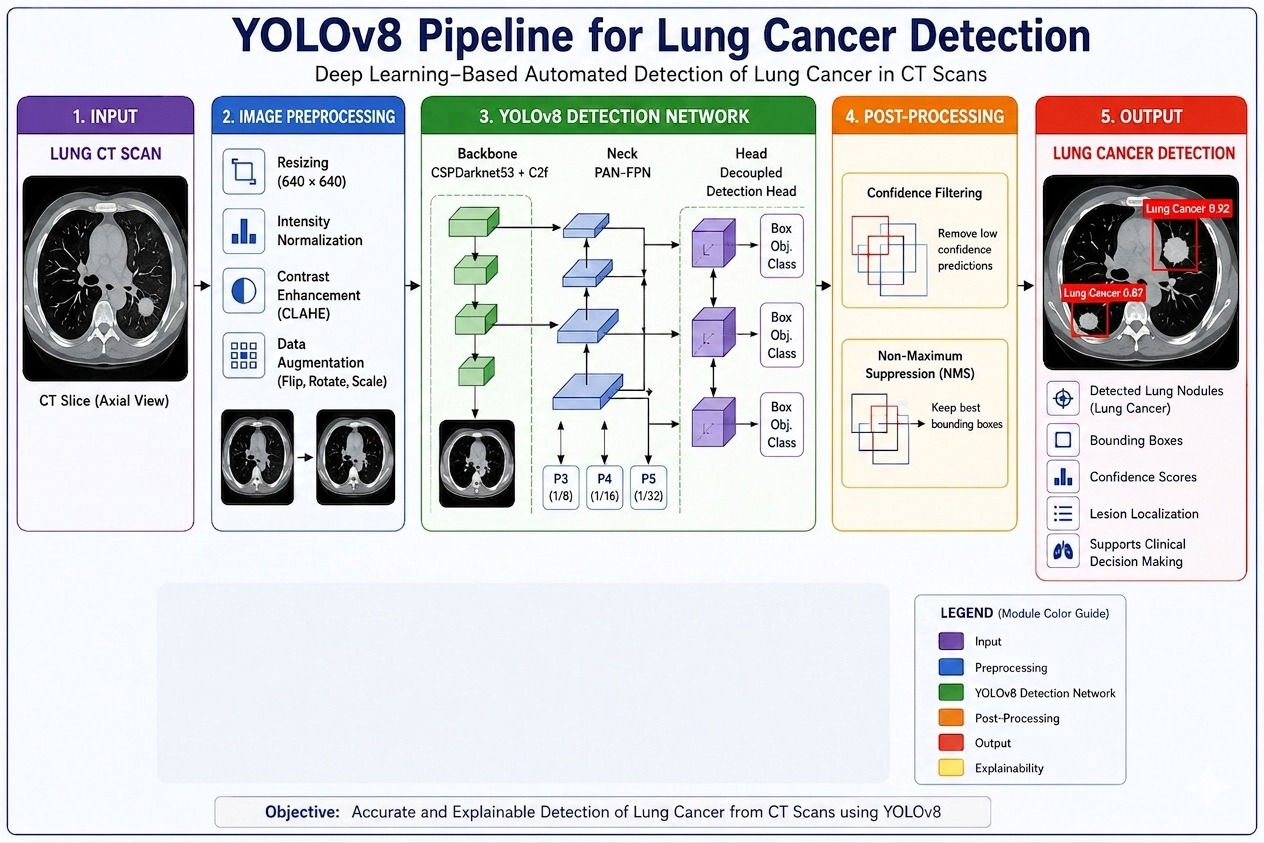
\includegraphics[width=\textwidth]{assets/yolo_arch.jpeg}
	\caption{Detailed architectural diagram of the YOLOv8 object detection framework, illustrating the Backbone, Neck (FPN + PAN), and Detection Head stages for multi-scale prediction.}
	\label{fig:yolov8_detailed_architecture}
\end{figure}

\subsubsection{Transfer Learning Strategy}
Training a deep object detector entirely from scratch typically requires extremely large medical imaging datasets. To overcome this limitation, transfer learning was employed. The detector was initialized using pretrained YOLOv8 weights trained on large-scale image datasets. The pretrained model already possesses strong low-level feature extraction capabilities, including detection of edges, contours, textures, and spatial patterns. Fine-tuning these representations on lung CT images significantly accelerates convergence while reducing the risk of overfitting.

\subsubsection{Training Configuration}
Model training was performed using the Ultralytics implementation of YOLOv8. The training pipeline automatically performs image loading, resizing, batching, label matching, loss computation, and weight optimization. Input images were resized to $640 \times 640$ pixels to ensure uniform tensor dimensions throughout training.

The optimization process simultaneously minimizes:
\begin{itemize}
	\item \textbf{Localization Loss:} Measures bounding-box accuracy.
	\item \textbf{Classification Loss:} Measures lesion classification accuracy.
	\item \textbf{Distribution Focal Loss (DFL):} Improves bounding-box regression precision.
\end{itemize}
The total loss is defined as:
\begin{equation}
	L_{\text{total}} = L_{\text{box}} + L_{\text{cls}} + L_{\text{DFL}}
\end{equation}
During training, stochastic gradient optimization updates network weights through backpropagation until convergence.